\subsection{Differenzverstärker} % (fold)
\label{sub:Differenzverstärker}
\begin{frame}
    \frametitle{Differenzverstärker}
    \framesubtitle{}
    \begin{figure}[H]
    \begin{center}
            \includegraphics[scale=0.2]{./img/schaltungen/differenz_einfach.png}
    \end{center}
    \end{figure}
\end{frame}
\begin{frame}
    \frametitle{Differenzverstärker: Bodediagramm}
    \framesubtitle{}
     \begin{figure}[H]
     \begin{center}
             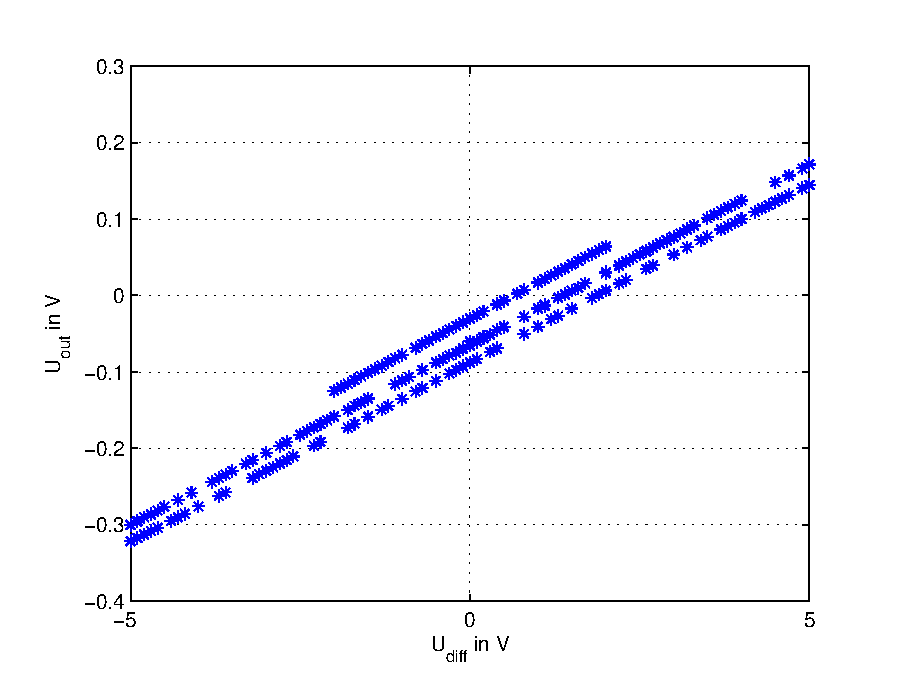
\includegraphics[scale=0.5]{./img/bode/Aufgabe_3_3_Ud.eps}
     \end{center}
     \end{figure}
\end{frame}
\begin{frame}
    \frametitle{Differenzverstärker: Bodediagramm}
    \framesubtitle{}
     \begin{figure}[H]
     \begin{center}
             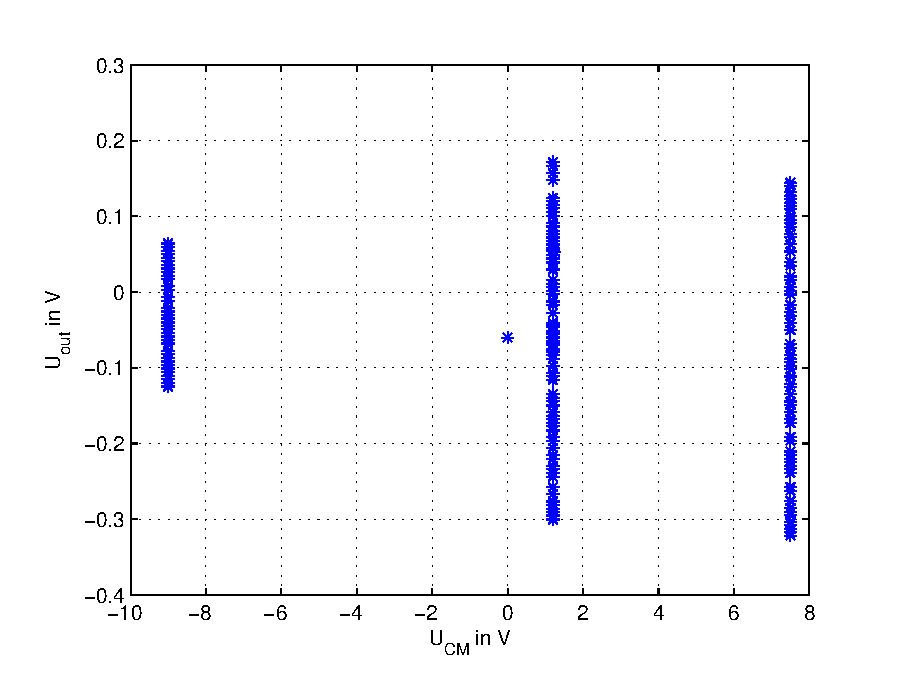
\includegraphics[scale=0.5]{./img/bode/Aufgabe_3_3_U.eps}
     \end{center}
     \end{figure}
\end{frame}
\begin{frame}
    \frametitle{Differenzverstärker}
    \framesubtitle{}
    \begin{figure}[H]
    \begin{center}
            \includegraphics[scale=0.2]{./img/schaltungen/differenz_optimiert.png}
    \end{center}
    \end{figure}
\end{frame}
\begin{frame}
    \frametitle{Optimierter Differenzverstärker: Bodediagramm}
    \framesubtitle{}
     \begin{figure}[H]
     \begin{center}
             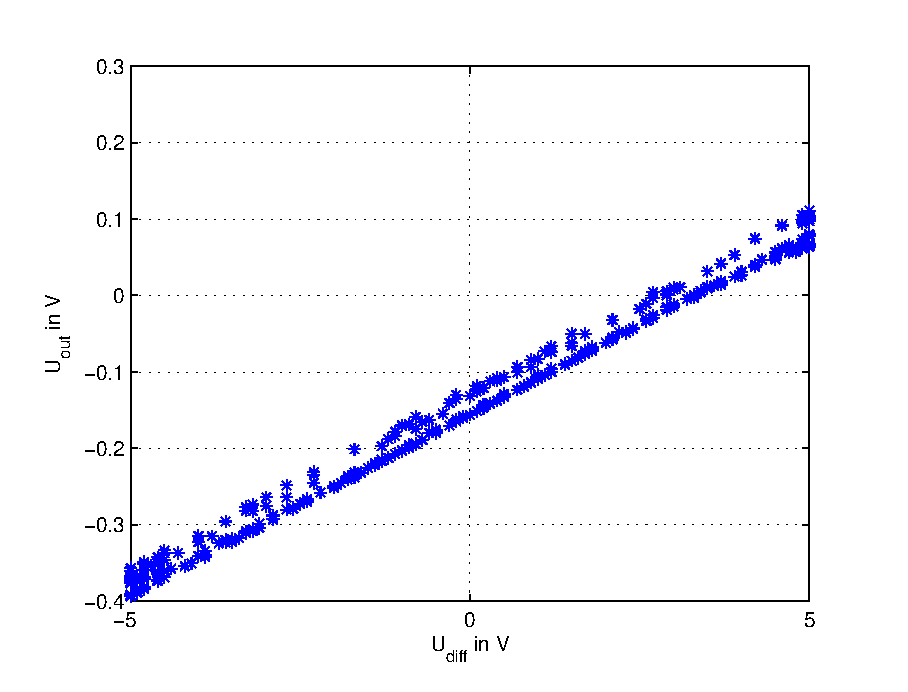
\includegraphics[scale=0.5]{./img/bode/Aufgabe_3_4_Ud.eps}
     \end{center}
     \end{figure}
\end{frame}
\begin{frame}
    \frametitle{Optimierter Differenzverstärker: Bodediagramm}
    \framesubtitle{}
     \begin{figure}[H]
     \begin{center}
             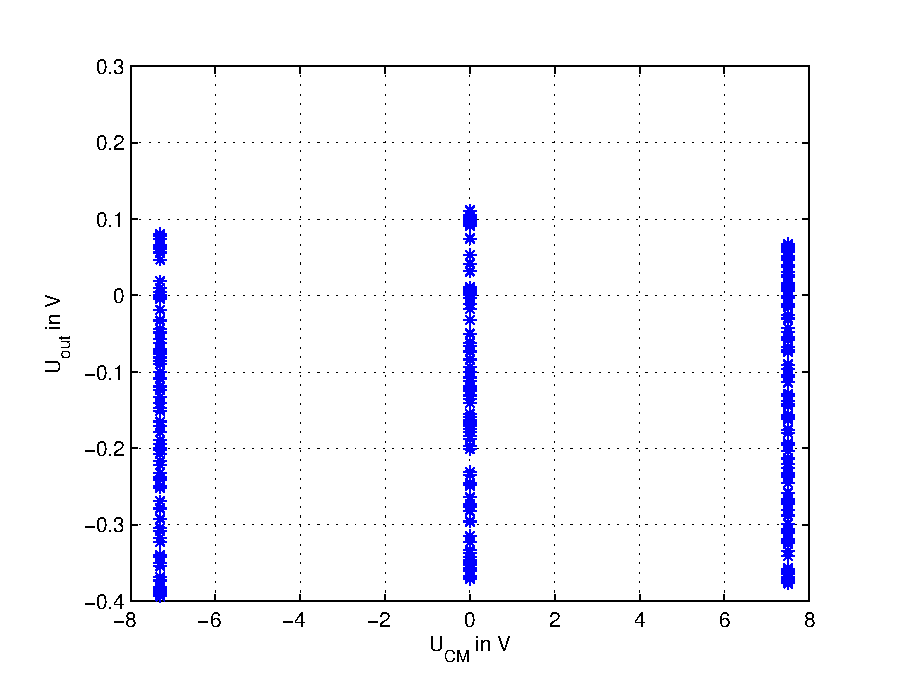
\includegraphics[scale=0.5]{./img/bode/Aufgabe_3_4_U.eps}
     \end{center}
     \end{figure}
\end{frame}
